
\documentclass[times,10pt,twocolumn]{article}



\usepackage{times}
\usepackage{pifont} 
\usepackage{import}
\usepackage{amsmath}
\usepackage{multirow}
\usepackage{graphicx,url}
\usepackage{placeins}
\usepackage{adjustbox}
\usepackage[english]{babel}
\usepackage{lipsum}
\usepackage{listings}
\usepackage[svgnames]{xcolor} 
\usepackage{caption}
\usepackage{amsmath}
\usepackage{calc} 
\usepackage{array,url,kantlipsum}
\usepackage{lscape}
\usepackage{array}
\usepackage{booktabs}
\usepackage{txfonts}
\usepackage{latex8}
\usepackage{colortbl}%
  \newcommand{\myrowcolour}{\rowcolor[gray]{0.925}}
\newenvironment{Figure}
  {\par\medskip\noindent\minipage{\linewidth}}
  {\endminipage\par\medskip}
  
\DeclareCaptionFont{white}{\color{white}}
\DeclareCaptionFormat{listing}{\colorbox[RGB]{60,100,180}{\parbox{0.40\textwidth - 2 \fboxsep}{\hspace{8pt}#1#2#3}}}
\captionsetup[lstlisting]{format=listing,labelfont=white,textfont=white, singlelinecheck=false, margin=0pt, font={bf,footnotesize}}

\pagestyle{empty}

\begin{document}



\title{Improving Stress Search Based Testing using a Hybrid Metaheuristic Approach}
\author{ Francisco Nauber Bernardo Gois\\
Servi\c{c}o Federal de\\
 Processamento de Dados\\
Avenida Pontes Vieria ,832\\
Fortaleza, Cear\'a, Brazil\\
francisco.gois@serpro.gov.br\\
\and
Pedro Porf\'irio Muniz de Farias\\
Universidade de Fortaleza\\
Av. Washington Soares, 1321\\
Fortaleza, Cear\'a, Brazil\\
porfirio@unifor.br\\
\and
Andr\'e Lu\'is Vasconcelos Coelho\\
Universidade de Fortaleza\\
Av. Washington Soares, 1321\\
Fortaleza, Cear\'a, Brazil\\
acoelho@unifor.br\\
\and 
Thiago Monteiro Barbosa\\
Servi\c{c}o Federal de\\
 Processamento de Dados\\
Avenida Pontes Vieria ,832\\
Fortaleza, Cear\'a, Brazil\\
thiago.monteiro@serpro.gov.br
}




\maketitle
\thispagestyle{empty}

\begin{abstract}
 Some software systems must respond to thousands or millions of concurrent requests. These systems must be properly tested to ensure that they can function correctly under the expected load. A common use of stress search-based testing is to find test scenarios that produce execution times that violate the timing constraints specified. The purpose of this paper is determine if hybrid algorithms are superior to single metaheuristics when solving stress testing problems and improve the process of stress testing with a tool that evolves the test model during its execution. The research proposes a hybrid metaheuristic approach that uses genetic algorithms, simulated annealing, and Tabu search algorithms for use in stress test models. A tool named IAdapter, a JMeter plugin used for performing search-based load, performance, or stress tests, was developed. Two experiments were conducted to validate the proposed approach. The first experiment was performed on an emulated component, and the second one was performed using an installed Moodle application. In both experiments, the use of a hybrid metaheuristic approach produced better fitness values. 
\end{abstract}



\Section{Introduction}

Many systems must support concurrent access by hundreds or thousands of users. Failure to scale users results in catastrophic failures and unfavorable media coverage \cite{Jiang2010}. 

The explosive growth of the Internet has contributed to the increased need for applications that perform at an appropriate speed. Performance problems are often detected late in the application life cycle, and the later they are discovered, the greater the cost to fix them \cite{Molyneaux2009}.

The use of stress testing is an increasingly common practice owing to the increasing number of users. In this scenario, the inadequate treatment of a workload generated by concurrent or simultaneous access, generated by system users, can result in highly critical failures and negatively affect the customers's perception of the company \cite{Draheim2006b} \cite{Jiang2010}. 

Stress testing determines the responsiveness, throughput, reliability, or scalability of a system under a given workload. The quality of the results of a system's load tests is closely linked to the implementation of the workload strategy. The performance of many applications depends on the load applied under different conditions. In some cases, performance degradation and failures arise only in stress conditions \cite{Garousi2010} \cite{Jiang2010}.

A stress test uses a set of workloads that consist of many types of usage scenarios and a combination of different numbers of users. A load is typically based on an operational profile. Different parts of an application should be tested on various parameters and stress conditions \cite{Babbar2011}. The correct application of a stress test should cover most parts of an application above the expected load conditions (stress test)\cite{Draheim2006b}.

A stress test usually lasts for several hours or even a few days and only tests a limited number of workloads. The major challenge is to find the workloads that expose a major number of errors and to discover the maximum number of users supported by an application under test \cite{Barna2011}. 

Search-based test is seen as a promising approach for verifying timing constraints \cite{Afzal2009a}. A common objective of a load search-based test is to find test scenarios that produce execution times that violate the specified timing constraints \cite{Sullivan}. 

We wish to determine if hybrid algorithms are superior to single metaheuristics when solving stress testing problem and and improve the process of stress testing with a tool that evolves the test model during its execution. The paper proposes the use of a hybrid metaheuristic approach that combines genetic algorithms, simulated annealing, and Tabu search algorithms in stress tests. A tool named IAdapter (www.iadapter.org), a JMeter plugin for performing search-based load tests, was developed. Two experiments were conducted to validate the proposed approach. The first experiment was performed on an emulated component, and the second one was performed using an installed Moodle application.

The remainder of the paper is organized as follows. Section 2 presents the research-proposed approach. Section 3 presents the IAdapter tool. Section 4 discusses the related work. Section 5 shows the results of two experiments performed using the IAdapter plugin. Conclusions and further work are presented in Section 6.

\Section{Improving Load, Performance, and Stress Search-Based Testing Using a Hybrid Metaheuristic Approach}

A large number of researchers have recognized the advantages and huge potential of building hybrid mathematical programming methods and metaheuristics. The main motivation for creating hybrid metaheuristics is to exploit the complementary character of different optimization strategies. In fact, choosing an adequate combination of algorithms can be the key to achieving top performance in solving many hard optimization problems \cite{Puchinger2005}.


The proposed solution makes it possible to create a model that evolves during the test. The proposed solution model uses genetic algorithms, Tabu search, and simulated annealing in two different approaches. The three algorithms were selected because they can use a common genotype representation. The first approach uses the three algorithms independently, and the second approach uses the three algorithms collaboratively (hybrid metaheuristic approach).

In the first approach , the algorithms do not share their best individuals among themselves. Each algorithm evolves in a separate way (Fig. \ref{fig:firstaproach}). The second approach uses the algorithms in a collaborative mode (hybrid metaheuristic). In this approach, the three algorithms share their best individuals found (Fig. \ref{fig:secondapproach}).

The next subsections present details about the used metaheuristic algorithms (genotype representation and fitness function).

\begin{figure}[h]
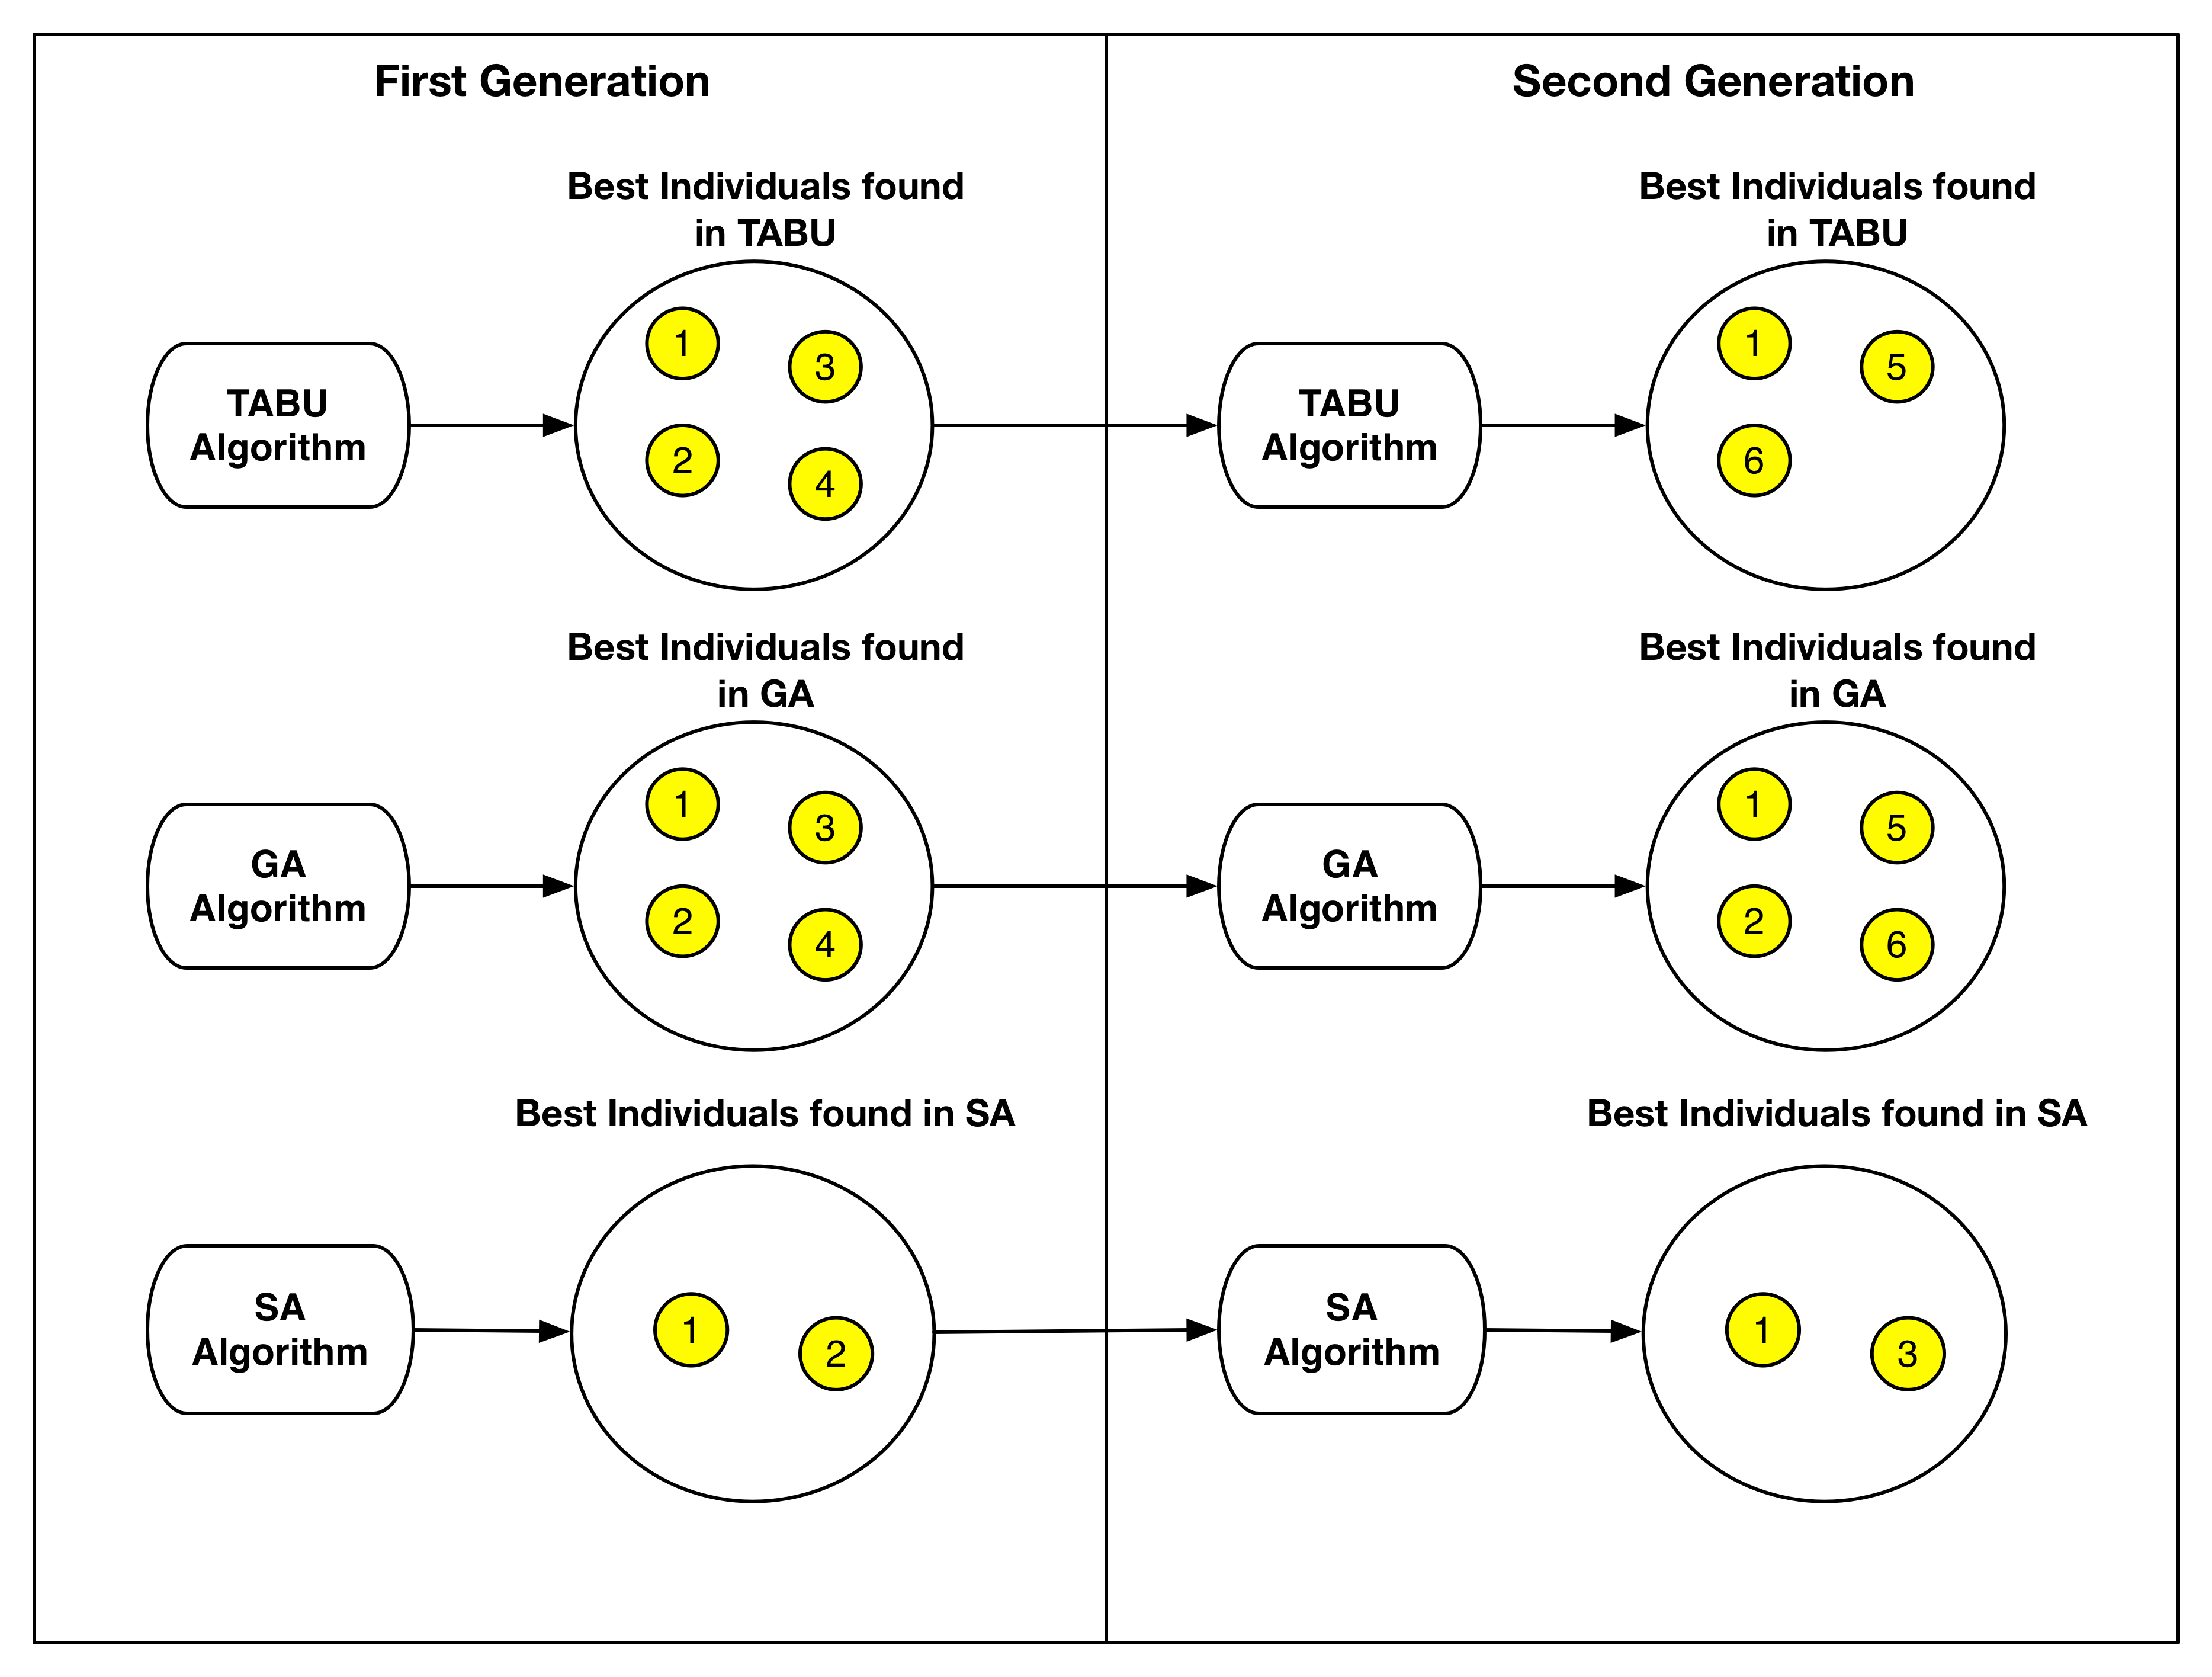
\includegraphics[width=0.5\textwidth]{./images/independ.png}
\caption{Use of the algorithms independently}
\label{fig:firstaproach}
\end{figure}
\begin{figure}
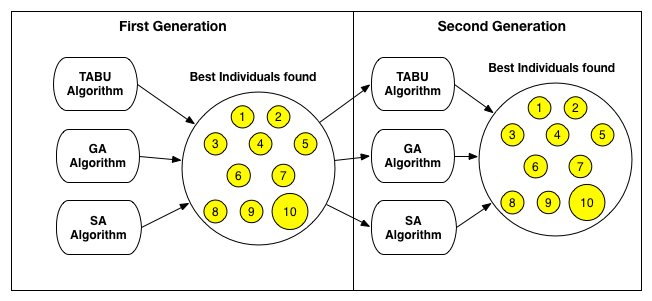
\includegraphics[width=0.5\textwidth]{./images/collaborative.png}
\caption{Use of the  algorithms collaboratively}
\label{fig:secondapproach}
\end{figure}

\SubSection{Genotype representation}

The genotype representation is composed by a linear vector with 23 genes. The first gene represents the name of an individual. The second gene represents the algorithm (genetic algorithm, simulated annealing, or Tabu search) used by the individual. The third gene represents the type of test. The next genes represent 10 scenarios and their numbers of users. Each scenario is an atomic operation: the scenario must log into the application, run the task goal, and undo any changes performed, returning the application to its original state.

Fig. \ref{fig:genomarepresentation} presents the genome representation and an example using the crossover operation. In the example, genotype 1 has the Login scenario with 2 users, the Form scenario with 0 users, and the Search scenario with 3 users. Genotype 2 has the Delete scenario with 10 users, the Search scenario with 0 users, and the Include scenario with 5 users. After the crossover operation, we obtain a genotype with the Login scenario with 2 users, the Search scenario with 0 users, and the Include scenario with 5 users.

\begin{figure}[h]
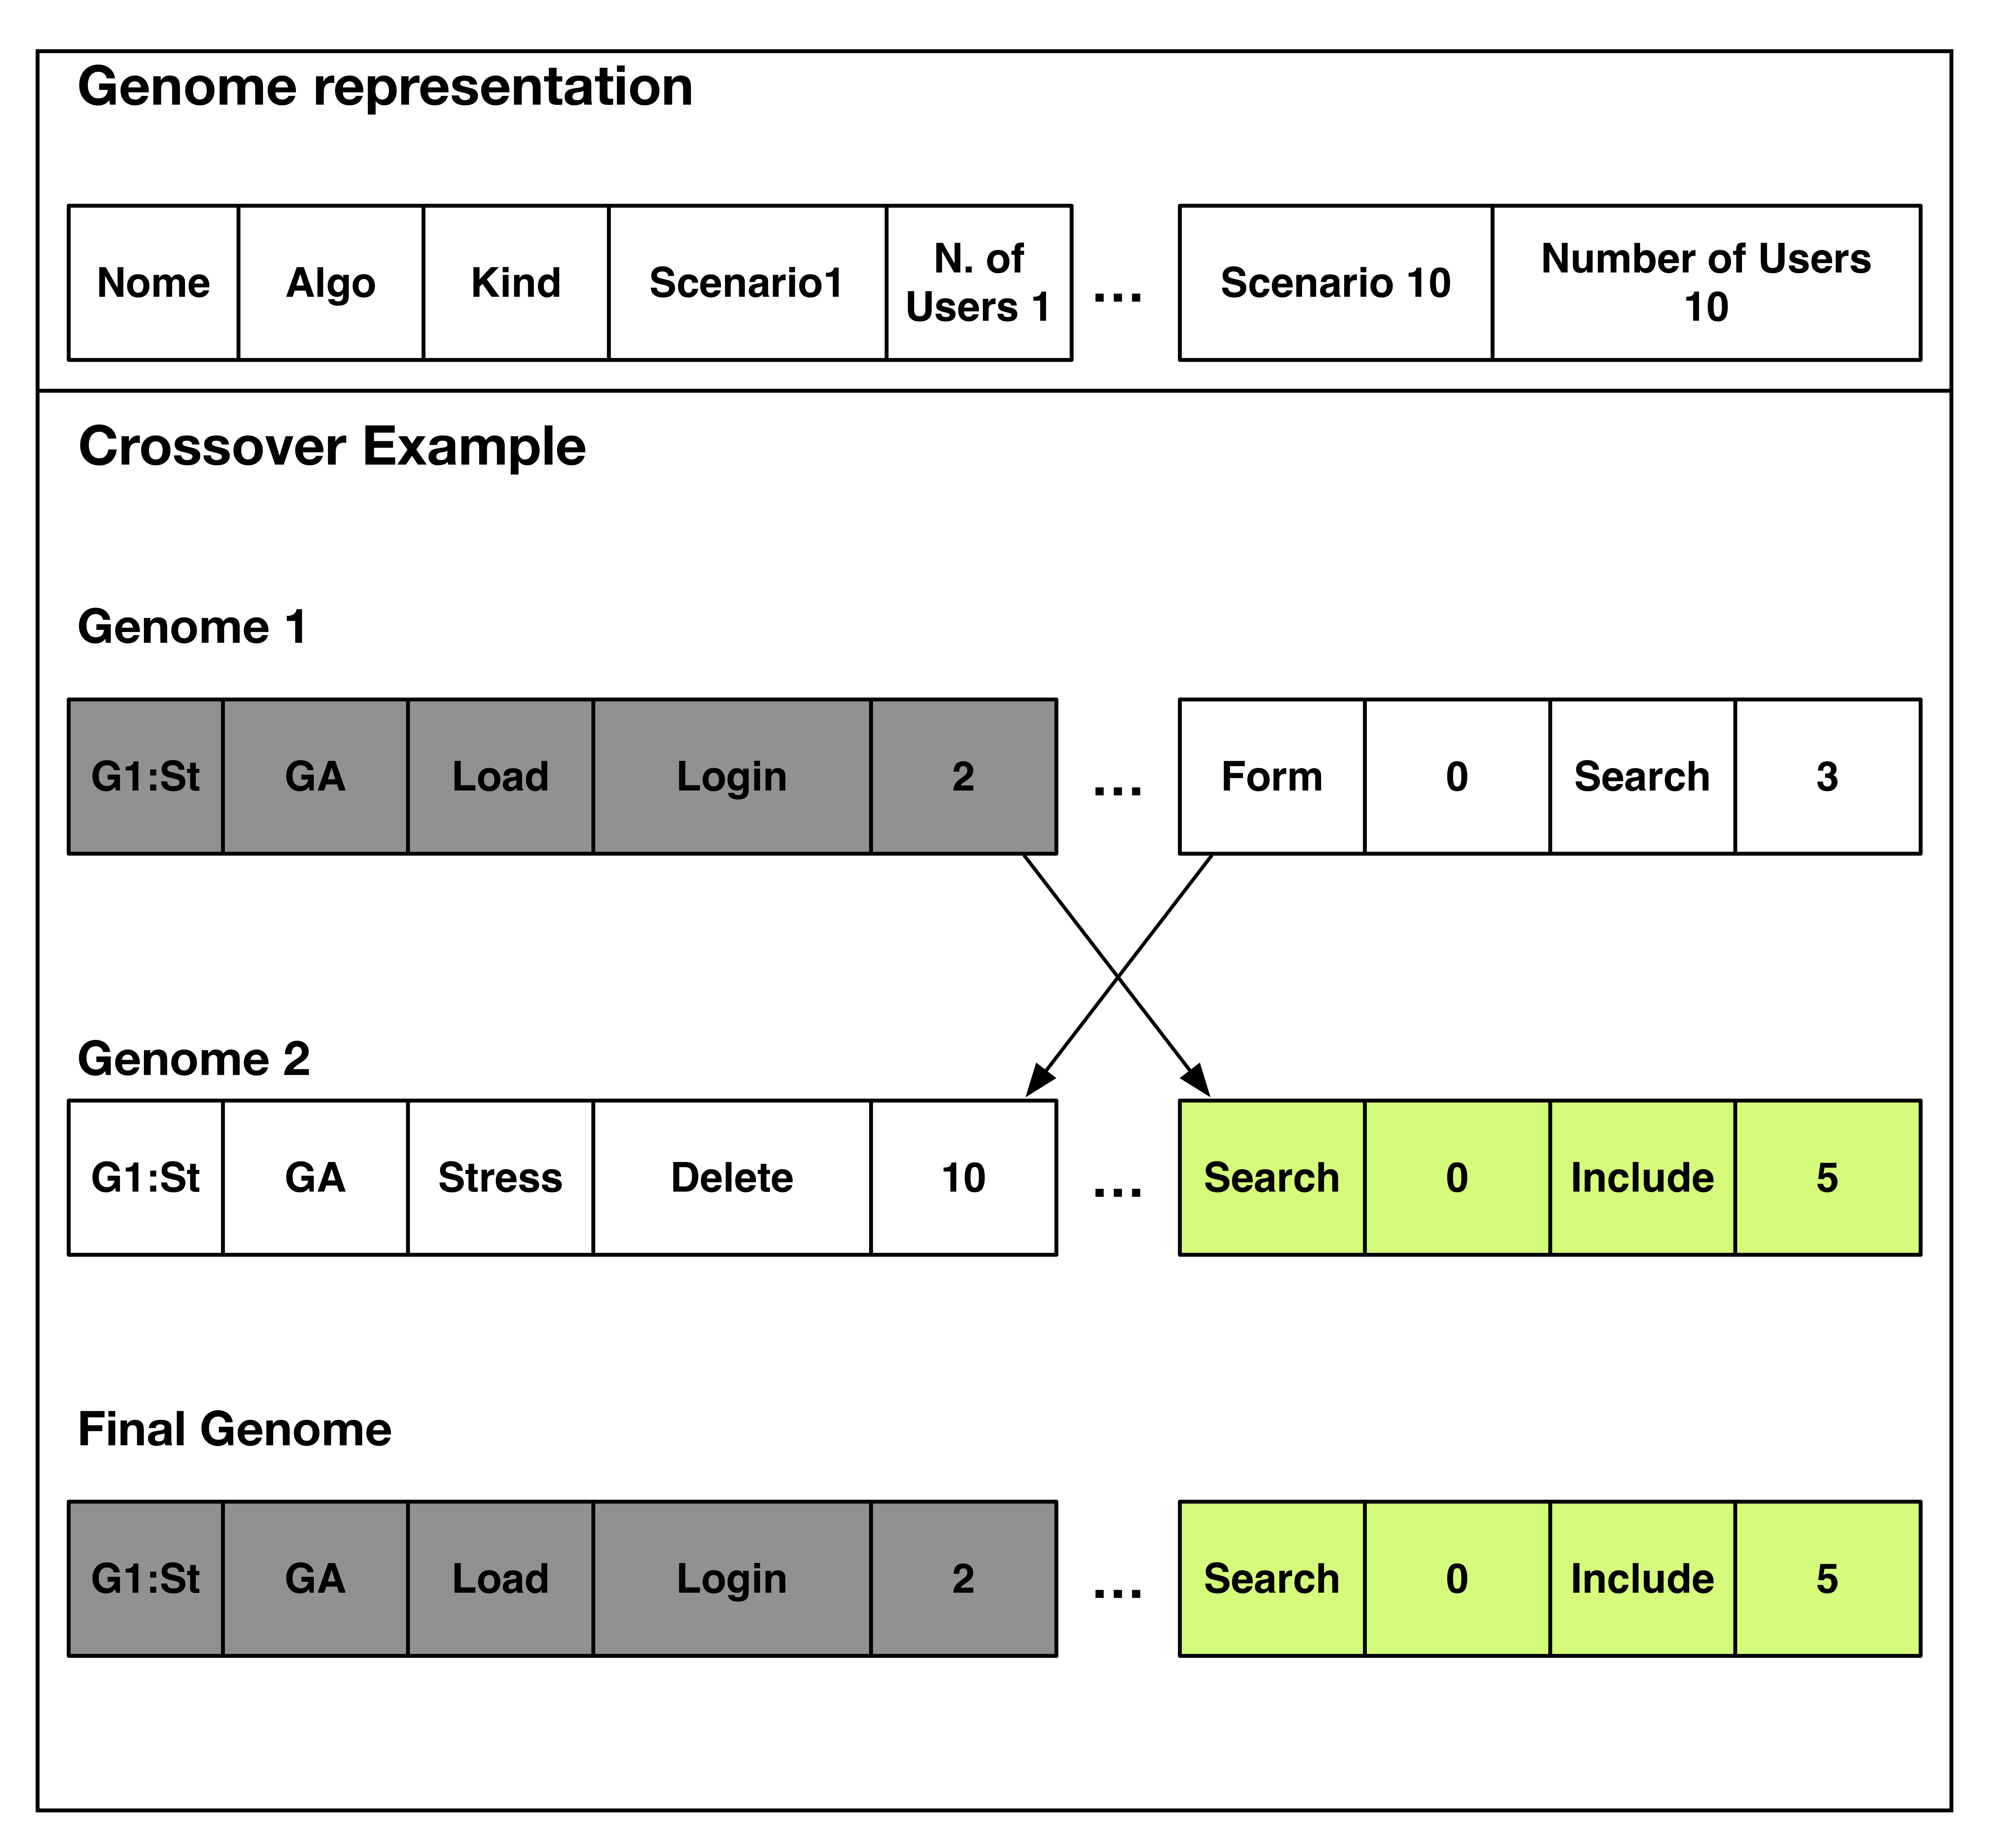
\includegraphics[width=0.5\textwidth]{./images/genomerepresentation.png}
\caption{Genotype representation and crossover example}
\label{fig:genomarepresentation}
\end{figure}

Fig. \ref{fig:neighbourtaby} shows the strategy used by the IAdapter tool to obtain the genotype of the neighbors for the Tabu search and simulated annealing algorithms. The neighbors are obtained by the modification of a single chromosome (scenario or number of users) in the genotype.


\begin{figure}[h]
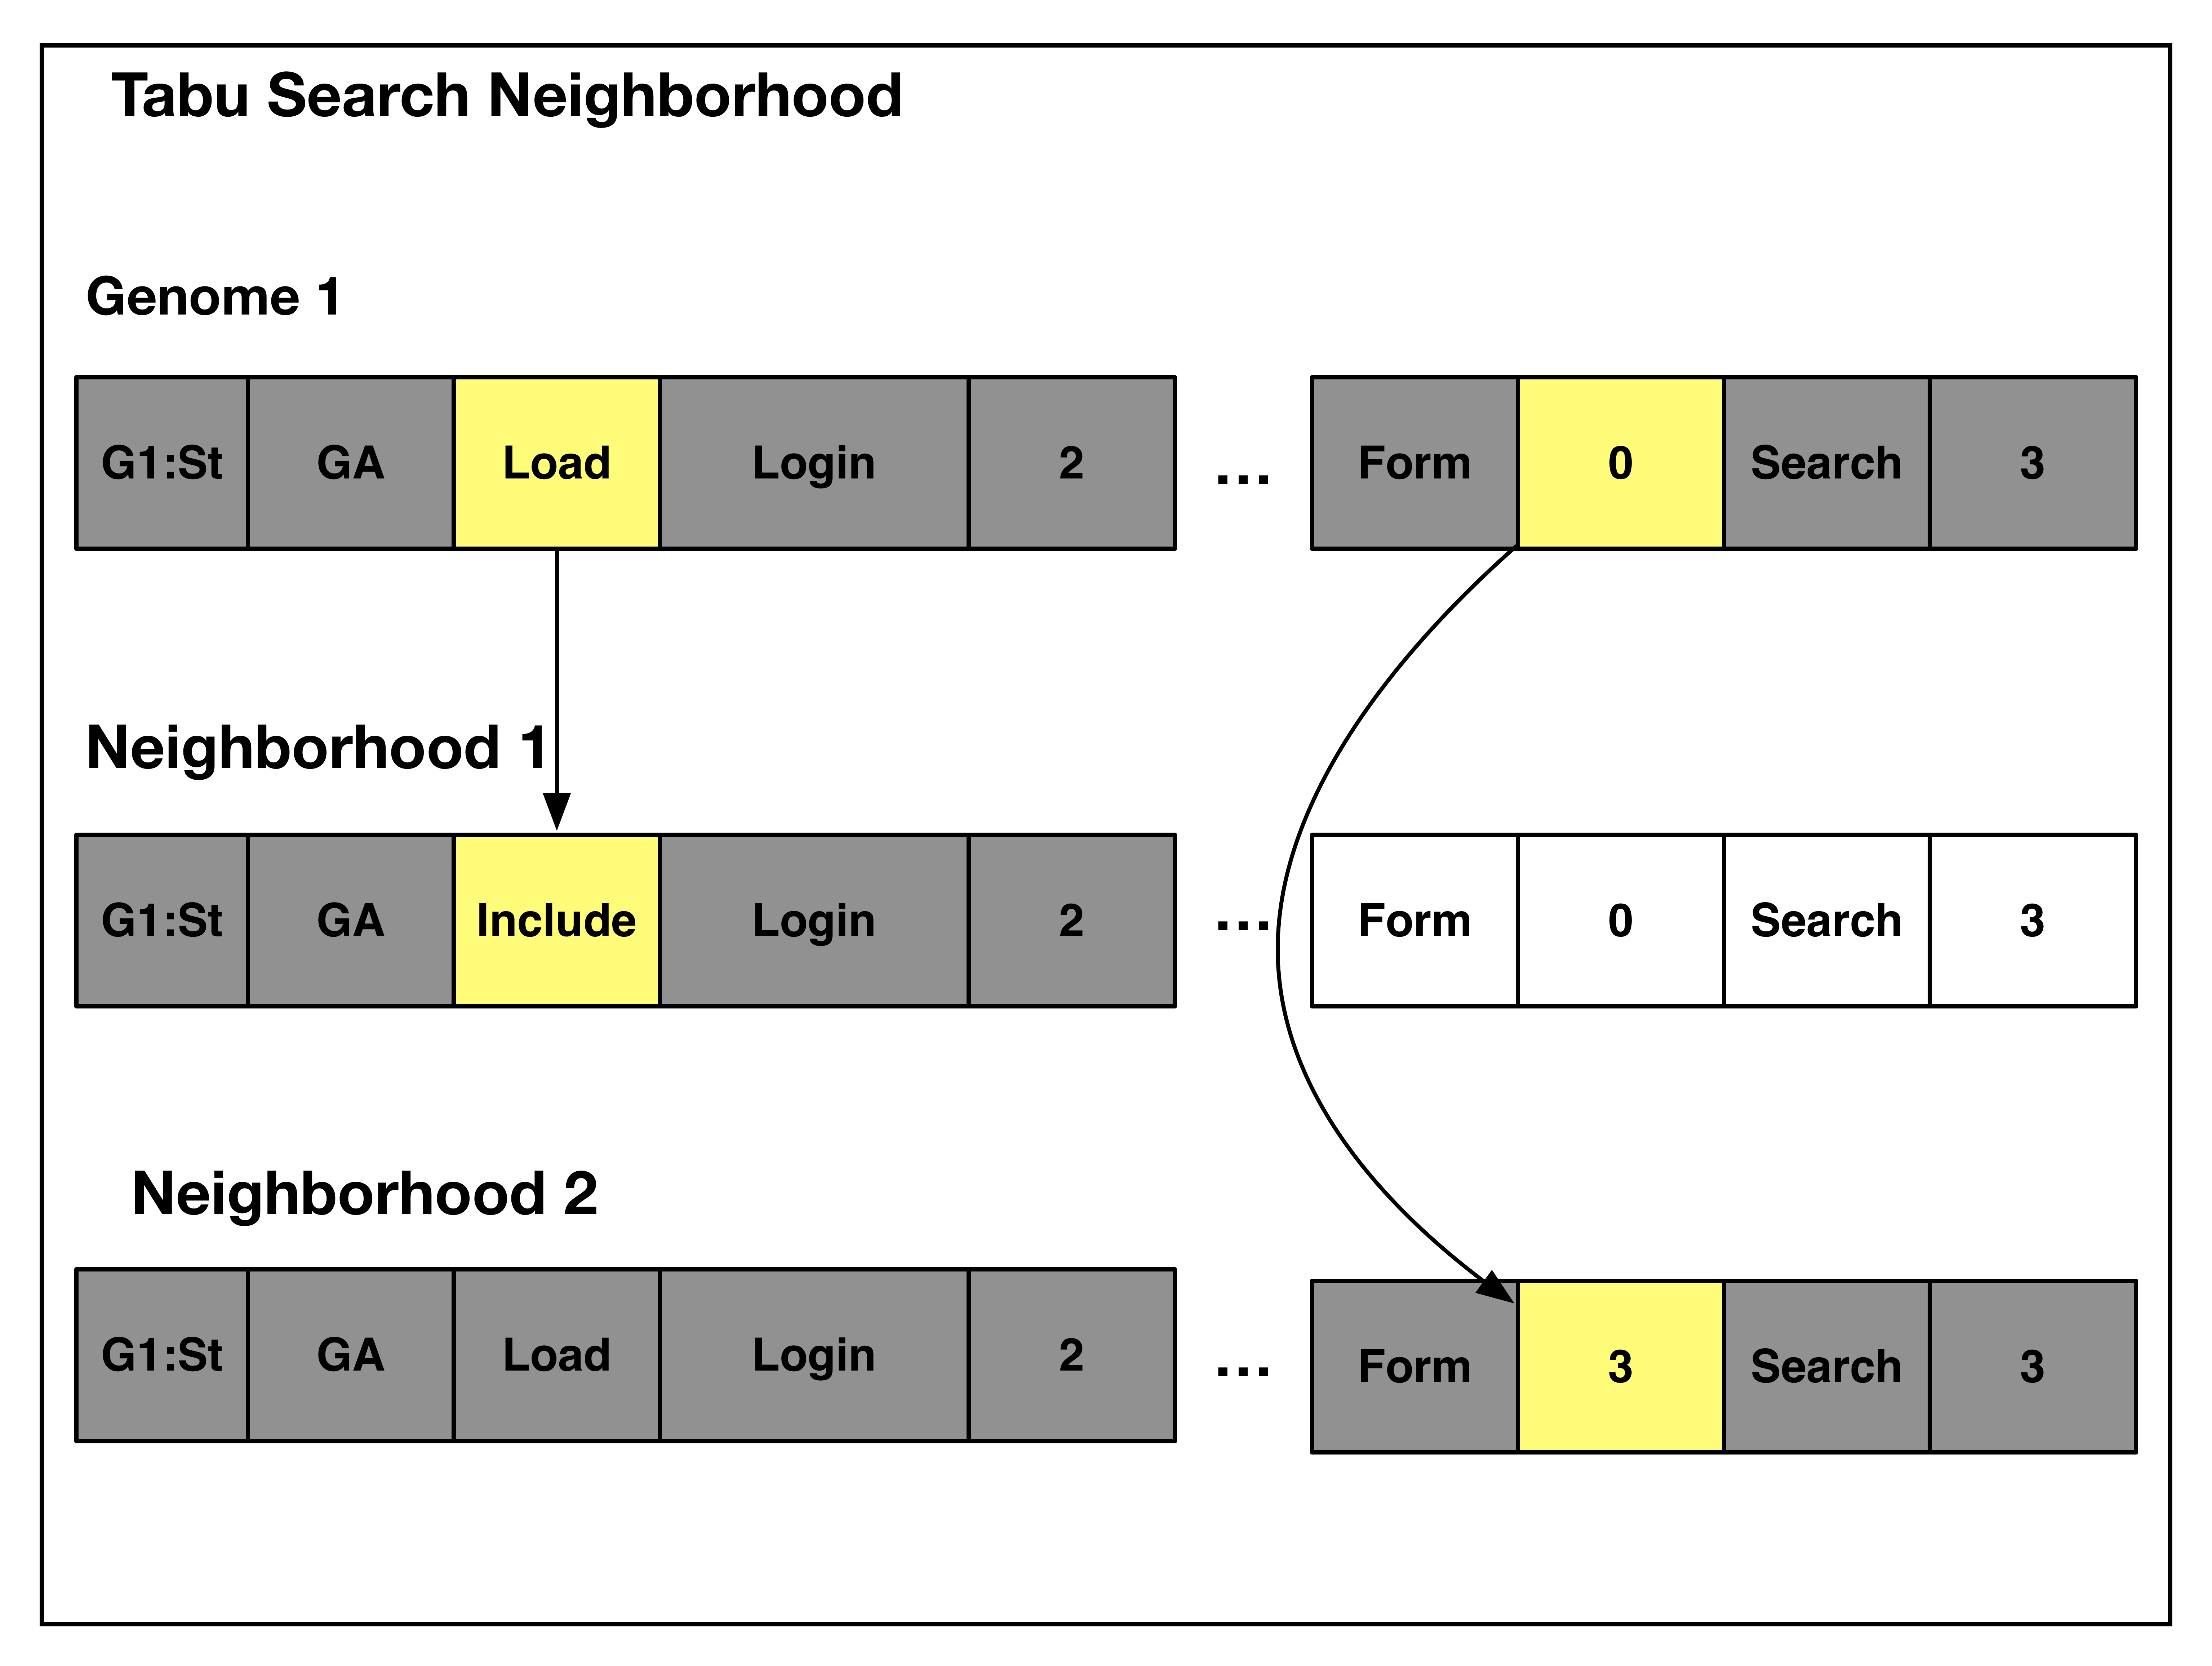
\includegraphics[width=0.5\textwidth]{./images/TabuNE.png}
\caption{Tabu search and simulated annealing neighbor strategy}
\label{fig:neighbourtaby}
\end{figure}

\SubSection{Objective (fitness) function}

The proposed solution uses the following equation as fitness function:

\begin{equation}
\begin{aligned}
fit=90percentileweigth* 90percentiletime\\
+80percentileweigth*80percentiletime\\+
70percentileweigth*70percentiletime+\\
maxResponseWeigth*maxResponseTime+\\
numberOfUsersWeigth*numberOfUsers-penalty
\end{aligned}
\end{equation}

The proposed solution uses 90,80 and 70-percentile. Some researchers advocate that the 90-percentile response time is a better measurement than the average/medium response time, as the former accounts for most of the peaks, while eliminating the outliers \cite{Jiang2010}. The proposed solution's fitness function uses a series of manually adjustable user-defined weights (90percentileweight, 80percentileweight,  70percentileweight, maxResponseWeight, and numberOfUsersWeight). These weights make it possible to customize the search plugin's functionality. A penalty is applied when an application under test takes a longer time to respond than the level of service.

\Section{IAdapter}

IAdapter is a JMeter plugin designed to perform search-based stress tests.  The plugin is available on www.iadapter.org. JMeter is a desktop application designed to test and measure the performance and functional behavior of applications. The IAdapter plugin implements the solution proposed in Section 2.

JMeter has components organized  in a hierarchical manner. The IAdapter plugin provides three main components: WorkLoadThreadGroup, WorkLoadSaver, and WorkLoadController.
 
WorkLoadThreadGroup is a component that creates an initial population and configures the algorithms used in IAdapter. The WorkLoadSaver component is responsible for saving all data in the database. The operation of the component only requires its inclusion in the test script. WorkLoadController represents a scenario of the test. All actions necessary to test an application should be included in this component. All instances of the component need to login to the application under test and return the application to its original state.

\Section{Related Work}

The search for the longest execution time is regarded as a discontinuous, nonlinear, optimization problem, with the input domain of the system under test as a search space \cite{Sullivan}. A common objective of search-based testing in stress tests is to find test scenarios that produce execution times that exceed the timing constraints specified. If a temporal error is found, the test was successful \cite{Sullivan}. The application of evolutionary algorithms to  stress tests involves finding the best- and worst-case execution times to determine whether timing constraints are fulfilled \cite{Afzal2009a}. There are two measurement units normally associated with the fitness function in stress test: processor cycles and execution time. The processor cycle approach describes a fitness function in terms of processor cycles. The execution time approach involves executing the application under test and measuring the execution time \cite{Afzal2009a} \cite{tracey2000search}.

Table \ref{tab:comparison}  shows a comparison between the presented research work and the research studies on load, performance, and stress tests presented by Afzal et al. \cite{Afzal2009a}. Afzal's work adds to some of the latest research in this area (\cite{Garousi2006} \cite{Garousi2010} \cite{DiAlesio2013} \cite{DiAlesio2014} \cite{Alesio2015}). The columns represent the type of tool used (prototype or functional tool), and the rows represent the metaheuristic approach used by each research study (genetic algorithm, Tabu search, simulated annealing, or a customized algorithm). The table also divides the research studies by the type of fitness function used (execution time or processor cycles). Most research studies are limited to making prototypes of genetic algorithms. The presented research work is distinguished from others by having a functional tool using a hybrid approach. 

The presented research work and Alesio's approach \cite{Alesio2015} use a hybrid approach with a functional tool. Whereas the present research uses an approach based on usage scenarios performing tests on an application installed in an available environment, Alesio uses sequence diagrams  to select for arrival time of tasks in systems from  safety-critical domains. 

\begin{table}[h]
\centering
\caption{Distribution of the research studies over the range of applied metaheuristics}
\label{tab:comparison}
\begin{tabular}{p{1.2cm}|p{1.8cm}|p{1.8cm}|p{1.8cm}|}
\cline{2-4}
                                                                & \multicolumn{2}{c|}{\textbf{Prototypes}}            & \textbf{Functional Tool} \\ \cline{2-4} 
                                                                & \begin{minipage}{0.2\textwidth}\footnotesize Execution Time  \end{minipage}          & \begin{minipage}{0.2\textwidth}\footnotesize Processor Cycles \end{minipage}        & \begin{minipage}{0.2\textwidth}\footnotesize Execution Time \end{minipage}           \\ \cline{2-4} 
%\setlength{\extrarowheight}{20pt}
\begin{tabular}[c]{@{}l@{}}\begin{minipage}{0.1\textwidth}\scriptsize GA + SA  \\ + Tabu \\ Search \end{minipage}\end{tabular}  & \cellcolor[HTML]{FFCCC9} & \cellcolor[HTML]{FFCCC9} & \cellcolor[HTML]{F8FF00} \begin{minipage}{0.2\textwidth} \scriptsize \textbf{  \\ IADAPTER \\} \end{minipage}  \\[2ex] \cline{2-4} 
\begin{minipage}{0.1\textwidth}\scriptsize GA \end{minipage}                                                              & \cellcolor[HTML]{CD9934} \begin{minipage}{0.12\textwidth}   \tiny \textnormal{ \\  Alander et al.,1998 \cite{Alander} \\ Wegener et al., 1996 and 1997 \cite{Wegener1997}\cite{J.WegenerK.GrimmM.GrochtmannH.Sthamer1996} \\  Sullivan et al., 1998 \cite{Sullivan} \\ Briand et al., 2005 \cite{Briand2005} \\ Canfora et al., 2005 \cite{Canfora}  \\ }\end{minipage} & \cellcolor[HTML]{CD9934} \begin{minipage}{0.12\textwidth} \tiny \textrm{  \\ Wegener and Grochtmann, 1998 \cite{Wegener1998} \\  Mueller et al., 1998 \cite{Mueller1998} \\ Puschner et al. \cite{Puschner1998} \\ Wegener et al., 2000 \cite{Stations} \\ Gro et al., 2000 \cite{Gross2000}  \\ }\end{minipage}& \cellcolor[HTML]{CD9934} \begin{minipage}{0.12\textwidth}   \tiny \textnormal{ \\  Di Penta, 2007 \cite{Penta2007} \\ Garoussi, 2006 \cite{Garousi2006} \\ Garousi, 2008 \cite{Garousi2008} \\ Garousi, 2010 \cite{Garousi2010} \\ } \end{minipage} \\[2ex] \cline{2-4} 
\begin{minipage}{0.1\textwidth}\scriptsize Simulated \\ Annealing \\ (SA) \end{minipage}                                                             & \cellcolor[HTML]{FFCCC9} & \cellcolor[HTML]{FFCCC9} & \cellcolor[HTML]{CD9934} \begin{minipage}{0.12\textwidth}   \tiny  Tracey, 1998 \cite{Tracey1998} \end{minipage} \\[2ex] \cline{2-4}
\begin{minipage}{0.1\textwidth}\scriptsize  Constraint \\ Programming \end{minipage}                                                             & \cellcolor[HTML]{FFCCC9} & \cellcolor[HTML]{FFCCC9} & \cellcolor[HTML]{CD9934} \begin{minipage}{0.12\textwidth}   \tiny  Alesio, 2014 \cite{DiAlesio2014} \\ Alesio, 2013 \cite{DiAlesio2013}  \end{minipage} \\[2ex] \cline{2-4} 
\begin{minipage}{0.1\textwidth}\scriptsize  GA +\\ Constraint \\ Programming \end{minipage}                                                             & \cellcolor[HTML]{FFCCC9} & \cellcolor[HTML]{FFCCC9} & \cellcolor[HTML]{CD9934} \begin{minipage}{0.12\textwidth}   \tiny  Alesio, 2015 \cite{Alesio2015} \end{minipage} \\[2ex] \cline{2-4} 
\setlength{\extrarowheight}{20pt}
\begin{tabular}[c]{@{}l@{}}
\begin{minipage}{0.1\textwidth}\scriptsize Customized \\ Algorithm \end{minipage}\end{tabular} & \cellcolor[HTML]{FFCCC9} & \cellcolor[HTML]{CD9934}  \begin{minipage}{0.12\textwidth}   \tiny  \textnormal{   \raggedleft Pohlheim, 1999 \cite{Pohlheim2005}  } \end{minipage} & \cellcolor[HTML]{FFCCC9} \\[4ex] \cline{2-4}
\end{tabular}
\end{table}



\Section{Experiments}

This section presents two experiments. The first one was performed on an emulated component, and the second one was performed using an installed Moodle application. The experiments used the following fitness function:

\begin{equation}
\begin{aligned}
fit=0.9* 90percentiletime\\
+0.1*80percentiletime\\+
0.1*70percentiletime+\\
0.1*maxResponseTime+\\
0.2*numberOfUsers-penalty
\end{aligned}
\end{equation}

This fitness function intended to find individuals with the highest percentile of 90\%, followed by individuals with a higher percentile time of 80\% and 70\%, maximum response time, and number of users. The first experiment implemented 27 generations, and the second experiment  performed 6 generations, with 300 executions by generation (100 times for each algorithm),  generating 300 new individuals. The experiments used an initial population of 100 individuals. The genetic algorithm used the top 10 individuals from each generation in the crossover operation. The Tabu list was configured with the size of 10 individuals and expired every 2 generations.  The mutation operation was applied to 10\% of the population on each generation. 

\SubSection{First Experiment: Emulated Class Test}

The first experiment aimed to perform performance, load, and stress testing on a simulated component. The purpose of using a simulated component was to be able to perform a greater number of generations in a shorter time available and eliminate variables such as the use of databases and application servers. The first experiment used a test class  named SimulateConcurrentAccess. This class has a static variable named \textit{x} and a set of methods that use the variable in a synchronized context.

Figure \ref{fig:results} presents the results obtained by the hybrid metaheuristic (HM) approach, genetic algorithm (GA), simulated annealing (SA), and Tabu search (TS) from 27 generations in the first experiment. The values are the maximum value of the fitness value obtained in each algorithm. A higher value in the figure means that the scenario has a greater response time by the application under test.  The signed-rank Wilcoxon non-parametrical procedure was used for comparing the results. The procedure showed that there was a significant improvement in the results using the three algorithms together.

\begin{figure}[h]
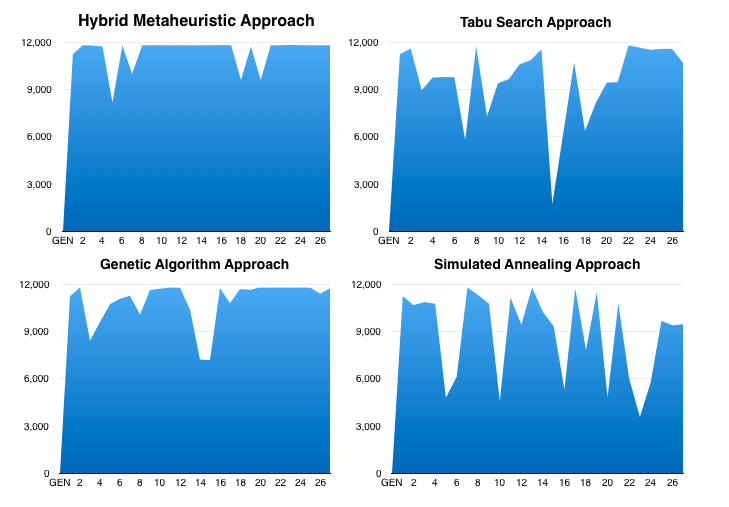
\includegraphics[width=0.5\textwidth]{./images/results.png}
\caption{Maximum value of the fitness function by algorithm}
\label{fig:results}
\end{figure}


\SubSection{Second Experiment: Moodle Application Test}

The second experiment used a Moodle application installed in a machine with 500 GB of hard disk space and 8 GB of memory. The study used six application scenarios:

\begin{itemize}
\item PostDeleteMessage: This scenario posts and deletes messages in the Moodle application.
\item MyHome: This scenario accesses the homepage of the user's application.
\item Login: This scenario is responsible for user authentication by the application.
\item Notifications: This scenario involves entering the notification page of each user.
\item Start Page: This scenario shows the initial start page of the application.
\item Badge: This scenario involves entering the badge page.
\end{itemize}

The maximum tolerated response time in the test was 30 seconds.  Any  individuals who obtained a time longer than the stipulated maximum time suffered penalties.  The whole process of stress and performance tests, which took 3 days and about 1800 executions, was carried out without the need for monitoring by a test designer. The tool automatically selected the next scenarios to be run up to the limit of six generations previously established. The small number of samples of the experiment is insufficient to give a statistical significance to the results of the Wilcoxon procedure. However, it is noted that, in four of six generations, the collaborative approach presented the best values. The experiment succeeded in finding 29 individuals whose maximum time expected by the application was obtained.  Table \ref{tab:secondexperiment1} shows an example of the six individuals with the highest fit values in the second experiment. The table shows the fitness value (Fit);  the name of the scenario (Scenario); the number of users (Users); and the percentiles of 90\%, 80\%, and 70\% (90per, 80per and 70per) in seconds.  


\begin{table}[h]
\centering
\caption{Example of individuals obtained in the second experiment}
\label{tab:secondexperiment1}
\begin{tabular}{|p{0.2cm}|l|l|l|p{0.60cm}|p{0.60cm}|p{0.60cm}|}
\hline
Id&Fit&Scenario&Users&90per&80per&70per\\ \hline
\multirow{2}{*}{1} & \multirow{2}{*}{35800} & MyHome        & 31              & \multirow{2}{*}{30} & \multirow{2}{*}{29} & \multirow{2}{*}{10} \\ \cline{3-4}
                   &                        & Badges        & 4               &                     &                     &                     \\ \hline
\multirow{3}{*}{2} & \multirow{3}{*}{35795} & MyHome        & 30              & \multirow{3}{*}{30} & \multirow{3}{*}{29} & \multirow{3}{*}{10} \\ \cline{3-4}
                   &                        & Notifications & 2               &                     &                     &                     \\ \cline{3-4}
                   &                        & Badges        & 2               &                     &                     &                     \\ \hline
\multirow{2}{*}{3} & \multirow{2}{*}{35782} & MyHome        & 32              & \multirow{2}{*}{30} & \multirow{2}{*}{29} & \multirow{2}{*}{10} \\ \cline{3-4}
                   &                        & Badges        & 3               &                     &                     &                     \\ \hline
\multirow{3}{*}{4} & \multirow{3}{*}{35773} & MyHome        & 22              & \multirow{3}{*}{30} & \multirow{3}{*}{29} & \multirow{3}{*}{10} \\ \cline{3-4}
                   &                        & Notifications & 6               &                     &                     &                     \\ \cline{3-4}
                   &                        & Badges        & 9               &                     &                     &                     \\ \hline
\multirow{2}{*}{5} & \multirow{2}{*}{35771} & MyHome        & 28              & \multirow{2}{*}{30} & \multirow{2}{*}{29} & \multirow{2}{*}{9}  \\ \cline{3-4}
                   &                        & Badges        & 6               &                     &                     &                     \\ \hline
\multirow{2}{*}{6} & \multirow{2}{*}{35683} & MyHome        & 27              & \multirow{2}{*}{30} & \multirow{2}{*}{29} & \multirow{2}{*}{8}  \\ \cline{3-4}
                   &                        & Badges        & 10              &                     &                     &                     \\ \hline
\end{tabular}
\end{table}





\Section{Conclusion}

This paper presented a hybrid metaheuristic approach for use in load, performance, and stress testing. Two experiments were performed to validate the solution. The first experiment was performed on an emulated component, and the second experiment was performed using an installed Moodle application.  The collaborative approach obtained better fit values in both experiments. 

The main contributions of this research are as follows: The presentation of a hybrid metaheuristic approach for use in  stress tests; the development of a JMeter plugin  for search-based tests; and  the automation of the load, performance, or stress test execution process. Among the future works of the research, the use of new combinatorial optimization algorithms such as very large-scale neighborhood search is one that we can highlight. 



%\section{Reference}
\bibliographystyle{latex8}
%\bibliographystyle{model1-num-names}
\bibliography{sample}
%\printbibliography
\end{document}
